%% RiSE Latex Template - version 0.5
%%
%% RiSE's latex template for thesis and dissertations
%% http://risetemplate.sourceforge.net
%%
%% (c) 2012 Yguaratã Cerqueira Cavalcanti (yguarata@gmail.com)
%%          Vinicius Cardoso Garcia (vinicius.garcia@gmail.com)
%%
%% This document was initially based on UFPEThesis template, from Paulo Gustavo
%% S. Fonseca.
%%
%% ACKNOWLEDGEMENTS
%%
%% We would like to thanks the RiSE's researchers community, the 
%% students from Federal University of Pernambuco, and other users that have
%% been contributing to this projects with comments and patches.
%%
%% GENERAL INSTRUCTIONS
%%
%% We strongly recommend you to compile your documents using pdflatex command.
%% It is also recommend use the texlipse plugin for Eclipse to edit your documents.
%%
%% Options for \documentclass command:
%%         * Idiom
%%           pt   - Portguese (default)
%%           en   - English
%%
%%         * Text type
%%           bsc  - B.Sc. Thesis
%%           msc  - M.Sc. Thesis (default)
%%           qual - PHD qualification (not tested yet)
%%           prop - PHD proposal (not tested yet)
%%           phd  - PHD thesis
%%
%%         * Media
%%           scr  - to eletronic version (PDF) / see the users guide
%%
%%         * Pagination
%%           oneside - unique face press
%%           twoside - two faces press
%%
%%		   * Line spacing
%%           singlespacing  - the same as using \linespread{1}
%%           onehalfspacing - the same as using \linespread{1.3}
%%           doublespacing  - the same as using \linespread{1.6}
%%
%% Reference commands. Use the following commands to make references in your
%% text:
%%          \figref  -- for Figure reference
%%          \tabref  -- for Table reference
%%          \eqnref  -- for equation reference
%%          \chapref -- for chapter reference
%%          \secref  -- for section reference
%%          \appref  -- for appendix reference
%%          \axiref  -- for axiom reference
%%          \conjref -- for conjecture reference
%%          \defref  -- for definition reference
%%          \lemref  -- for lemma reference
%%          \theoref -- for theorem reference
%%          \corref  -- for corollary reference
%%          \propref -- for proprosition reference
%%          \pgref   -- for page reference
%%
%%          Example: See \chapref{chap:introduction}. It will produce 
%%                   'See Chapter 1', in case of English language.

\documentclass[en,twoside,onehalfspacing,bsc]{risethesis}

\usepackage[english]{babel}
\usepackage{colortbl}
\usepackage{color}
\usepackage[table]{xcolor}
\usepackage{microtype}
\usepackage{bibentry}
\usepackage{subfigure}
\usepackage{multirow}
\usepackage{rotating}
\usepackage{booktabs}
\usepackage{pdfpages}
\usepackage{caption}
\usepackage{lipsum}

\captionsetup[table]{position=top,justification=centering,width=.85\textwidth,labelfont=bf,font=small}
\captionsetup[lstlisting]{position=top,justification=centering,width=.85\textwidth,labelfont=bf,font=small}
\captionsetup[figure]{position=bottom,justification=centering,width=.85\textwidth,labelfont=bf,font=small}

%% Change the following pdf author attribute name to your name.
\usepackage[linkcolor=black,
            citecolor=blue,
            urlcolor=black,
            colorlinks,
            pdfpagelabels,
            pdftitle={Rise Thesis Template (ABNT)},
            pdfauthor={Rise Thesis Template (ABNT)}]{hyperref}

\address{RECIFE}

\universitypt{Universidade Federal Rural de Pernambuco}
\universityen{Federal Rural University of Pernambuco}

\departmentpt{Departamento de Estatística e Informática}
\departmenten{Department of Statistics and Informatics}

\programpt{Bacharelado em Ciência da Computação}
\programen{BsC in Computer Science}

\majorfieldpt{Ciência da Computação}
\majorfielden{Computer Science}

\title{Evolutionary Approaches to Multi Agent Timed Patrolling}

\date{2015}

\author{Vítor de Albuquerque Torreão}
\adviser{Pablo Azevedo Sampaio}
% \coadviser{Eduardo Santana de Almeida}

% Macros (defines your own macros here, if needed)
\def\x{\checkmark}

\begin{document}

\frontmatter

\frontpage

\presentationpage

\begin{fichacatalografica}
	\FakeFichaCatalografica % Comment this line when you have the correct file
%     \includepdf{fig_ficha_catalografica.pdf} % Uncomment this
\end{fichacatalografica}

\banca

\begin{dedicatory}
I dedicate this work to all my family, friends and professors who gave me the
necessary support to get here.
\end{dedicatory}

\acknowledgements
Agradeço aos meus pais, Roberto e Cláudia por terem investido tudo em mim e me 
ensinado desde cedo a valorizar a minha educação.

Agradeço a minha irmã, Maria da Graça, pela ajuda com o seu silêncio dentro de 
casa enquanto redigia e pelo seu super poder de me deixar mais confiante.

Agradeço a minha querida e amada companheira, Marília, que me aturou nos 
momentos de estresse, incerteza e ansiedade durante toda a faculdade e 
especialmente enquanto trabalhava nesta monografia.

Meus sinceros agradecimentos a todos os professores do curso de Bacharelado em 
Ciência da Computação da Universidade Federal Rural de Pernambuco que me ajudaram 
nesta caminhada fantástica pelo ensino superior.

Finalmente, agradeço a Deus pela calma e clareza de raciocínio que me foram 
dadas quando mais precisava, não só nesta, mas em todas as provações que passei.

\begin{epigraph}[]{Albert Einstein}
Not everything that counts can be counted, and not everything that can be counted counts.
\end{epigraph}

\resumo
% Escreva seu resumo no arquivo resumo.tex
O gerenciamento eficiente de solicitações de mudança (SM) é fundamental para o
sucesso das atividades de manutenção e evolução de software. Entretanto, a
atribuição de SMs a desenvolvedores de software é um aspecto custoso desse
gerenciamento, pois demanda tempo e requer conhecimento apropriado do projeto de
software. Com o propósito de diminuir esse custo, várias pesquisas já propuseram
métodos de atribuição automática de SMs. Embora representem avanços na área,
existem vários fatores inerentes a atribuição de SMs que não são considerados
nessas pesquisas e são essenciais para a automação.

Como demonstrado nesse trabalho, a atribuição automática deve, por exemplo,
considerar a carga de trabalho, a experiência e o conhecimento dos
desenvolvedores, a prioridade e a severidade das SMs, a afinidade dos
desenvolvedores com os problemas descritos nas SMs, e até mesmo os
relacionamentos interpessoais. Para tornar esse cenário ainda mais complexo,
esses fatos podem variar de acordo com o projeto de software que está sendo
desenvolvido. Assim, uma solução para o problema de atribuição de SMs depende de
informações contextuais.

Assim, esse trabalho propõe, implementa e valida uma solução arquitetural
sensível ao contexto para atribuição automática de SMs. Dado o aspecto
contextual da solução, a arquitetura enfatiza a necessidade de considerar as
diversas fontes de informações presentes na organização, assim como a
necessidade de se desenvolver algorítimos que implementem diferentes estratégias
de atribuição. A proposta e implementação dessa solução é embasada em resultados
de duas pesquisas quantitativas: um estudo de mapeamento sistemático da
literatura, e uma pesquisa de questionário com desenvolvedores de software. Esse
último forneceu um conjunto de requisitos que a solução automatizada deve
satisfazer para que as estratégias de atribuição sejam atendidas, enquanto o
mapeamento da literatura identificou técnicas, algoritmos, e outros requisitos
necessários a automação.

A implementação da arquitetura segue uma estratégia de automação, também
elabo\-rada nesse trabalho, que possui dois componentes principais: um sistema
especialista baseado em regras (SEBR); e um modelo de recuperação de informação
(MRI) com técnicas de aprendizagem. Em nossa estratégia, esses dois componentes
são executados alternadamente em momentos diferentes a fim de atribuir uma SM
automaticamente. O SEBR processa regras simples e complexas, considerando
informações contextuais do projeto de software e da organização que o
desenvolve. O MRI é utilizado para fazer o casamento entre SMs e desenvolvedores
de acordo com o histórico de atribuições.

\begin{keywords}
Engenharia de Software, Manutenção e Evolução de Software, Gerenciamento de
Solicitações de Mudança, Atribuição Automática de Solicitações de Mudança
\end{keywords}

\abstract
% Write your abstract in a file called abstract.tex
The Multiagent Temporal Patrolling is a complex multi-agent task, which requires 
a group of agents to coordinate each other’s actions in order to obtain optimal 
results for the whole group. Patrolling a country’s borders, watching the 
corridors of a building, monitoring maritime fleets, inspecting areas that may be 
subject to gas leakage or fires are examples of such a patrolling task. An 
efficient solution to the Multiagent Patrolling can contribute in a variety of 
domains such as computer network administration, web search engines and traffic 
inspection.

Previous works have proposed many solutions to patrolling efficiently with a group 
of agents. Heuristic agents, game theory based agents, negotiation mechanisms, 
decision-making mechanisms, reinforced learning techniques, gravitational strategies, 
ant colony based agents and hybrid evolutionary approaches have all been applied to 
solve the multi agent patrolling problem. This work aims to contribute to the study 
of the patrolling task by developing a pure evolutionary approach and comparing it 
to other strategies proposed in the literature through simulations.

The empirical evaluation of the strategies will be made using benchmarks proposed by 
other researchers in traditional publications, software freely available on the 
internet and maintained by the community of researchers, and the patrolling simulator 
named Simple Patrol provided by researchers from the 
Universidade Federal Rural de Pernambuco.

\begin{keywords}
autonomous agents, multi agent systems, coordination and patrolling, evolutionary 
algorithms
\end{keywords}

% List of figures
\listoffigures

% List of tables
\listoftables

% List of acronyms
% Acronyms manual: http://linorg.usp.br/CTAN/macros/latex/contrib/acronym/acronym.pdf
\listofacronyms
\begin{acronym}[ACRONYM] 
% Change the word ACRONYM above to change the acronym column width.
% The column width is equals to the width of the word that you put.
% Read the manual about acronym package for more examples:
%   http://linorg.usp.br/CTAN/macros/latex/contrib/acronym/acronym.pdf
%\acro{afm}[AFM]{Alphabet Frequency Matrix}
%\acro{api}[API]{Application Programming Interface}
%\acro{arima}[ARIMA]{Auto-Regressive Integrated Moving Average}
%\acro{brn}[BRN]{Bug Report Network}
%\acro{bts}[BTS]{Bug Triage System}
%\acro{cas}[CAS]{Context-Aware Systems}
%\acro{ccb}[CCB]{Change Control Board}
%\acro{cr}[CR]{Change Request}
%\acro{cvs}[CVS]{Concurrent Version System}
%\acro{es}[ES]{Expert System}
%\acro{floss}[FLOSS]{Free/Libre Open Source Software}
%\acro{glr}[GLR]{Generalized Linear Regression}
%\acro{gqm}[GQM]{Goal Question Metric}
%\acro{html}[HTML]{HyperText Markup Language}
%\acro{ir}[IR]{Information Retrieval}
%\acro{irt}[IRT]{Recôncavo Institute of Technology}
%\acro{jdt}[JDT]{Jazz Duplicate Finder}
%\acro{lda}[LDA]{Latent Dirichlet Allocation}
%\acro{loc}[LOC]{Lines of Code}
%\acro{lsi}[LSI]{Latent Semantic Indexing}
%\acro{ms}[MS]{Mapping Study}
%\acro{msr}[MSR]{Mining Software Repositories}
%\acro{nlp}[NLP]{Natural Language Processing}
%\acro{promise}[PROMISE]{Predictive Models in Software Engineering}
%\acro{rbes}[RBES]{Rule-Based Expert System}
%\acro{rhel}[RHEL]{RedHat Enterprise Linux}
%\acro{saas}[SaaS]{Software as a Service}
%\acro{scm}[SCM]{Software Configuration Management}
%\acro{serpro}[SERPRO]{Brazilian Federal Organization for Data Processing}
%\acro{slr}[SLR]{Stepwise Linear Regression}
%\acro{slr}[SLR]{Systematic Literature Review}
%\acro{svd}[SVD]{Singular Value Decomposition}
%\acro{svm}[SVM]{Support Vector Machine}
%\acro{svn}[SVN]{Subversion}
%\acro{tfidf}[TF-IDF]{Term Frequency-Inverse Document Frequency}
%\acro{vsm}[VSM]{Vector Space Model}
%\acro{xp}[XP]{Extreming Programming}
\acro{tmap}[TMAP]{Timed Multiagent Patrolling}
\acro{tsp}[TSP]{Problema do Caixeiro Viajante}
\acro{ea}[EA]{Algoritmos Evolucionários}
\acro{aco}[ACO]{\textit{Ant Colony Optimization}}
\acro{es}[ES]{Estratégia Evolucionária}
%\acro{de}[DE]{Evolução Diferencial}
\acro{ga}[GA]{Algoritmo Genético}
\end{acronym}

% Summary (tables of contents)
\tableofcontents

\mainmatter

\chapter{Introdução}
\label{chp:introduction}

% \begin{quotation}[]{Poul Anderson}
% I have yet to see any problem, however complicated, which, when looked at in the
% right way, did not become still more complicated.
% \end{quotation}

Atividades relacionadas à vigilância, inspeção e controle, que hoje são 
realizadas por seres humanos, são candidatas a serem executadas por sistemas 
autônomos no futuro \citep{hernandez2013game}. Alguns exemplos dessas tarefas 
são: patrulhar fronteira de países ou muros de uma área civil, vigiar os 
corredores de um prédio, monitorar frotas marítimas e inspecionar áreas sujeitas 
a vazamentos de gás ou incêndios \citep{sampaiophd}.

Segundo a publicação \citep{hernandez2013game}, esses sistemas de segurança 
quando operados por humanos são, em sua maioria, previsíveis e inflexíveis, pois 
sua performance pode ser influenciada por fatores como o tédio, a distração ou a 
fadiga. Dessa forma, os autores afirmam que é importante melhorar os elementos 
de segurança desses sistemas para auxiliar seres humanos e destacam a Patrulha 
Multiagente \citep{Chevaleyre:2004:TAM:1018411.1019013} como um dos sistemas que 
pode fazer esse papel.

A Patrulha Multiagente pode ser definida como a tarefa de um agente que deve 
perceber uma porção limitada do ambiente e detectar eventos ou anomalias 
\citep{6315145}. Mais especificamente, pode ser definida como um problema no qual 
um time de indivíduos (agentes), visita tão frequentemente quanto possível, 
pontos de interesse contidos em uma área \citep{6495145}. Ou ainda como um 
problema de vigilância, onde deve-se minimizar o tempo entre visitas dos agentes 
aos locais importantes de um ambiente conhecido 
\citep{Pippin:2013:PBT:2480362.2480378}.

Existem algumas versões do problema que estendem essa definição, variando as 
características dos agentes e do ambiente. Dentre elas destacam-se: problema da 
patrulha em ambientes dinâmicos, isto é, o ambiente onde o agente se move muda 
ao longo da execução do agente \citep{6615158}. Outra variação leva em 
consideração que os agentes podem ter velocidades diferentes \citep{6900280}. 
Alguns autores trabalharam com o problema da patrulha onde os agentes não tem a 
mesma capacidade e operam em diferentes níveis de qualidade 
\citep{Pippin:2013:PBT:2480362.2480378}. Outros trabalham com agentes que 
possuem restrições de mobilidade \citep{6315145}. E há ainda uma variação onde a 
quantidade de agentes muda ao longo da execução, isto é, um determinado agente 
pode sair ou ser substituído por outro: são os chamados sistemas abertos 
\citep{6495145}.

Para estudar o problema, no entanto, esta pesquisa utilizará uma definição mais 
formal, precisa e abrangente do problema, que auxilie o pesquisador a enxergar 
a patrulha multiagente do ponto de vista matemático e a implementar soluções em 
aplicações de software. Assim, a definição técnica empregada no decorrer deste 
trabalho será a proposta por Sampaio \citep{sampaiophd}.

Segundo o autor, uma instância da Patrulha Multiagente Temporal, do inglês 
\ac{tmap}, é uma 7-tupla, $ \langle E, P, S, s_{0}, A, I, M \rangle $. O 
ambiente que o agente percebe é representado por um grafo 
\citep{Rosen:2002:DMA:579402}, $E$, onde os vértices representam os pontos de 
interesse, $P$, a serem visitados e as arestas representam os caminhos entre 
esses pontos. Na \figref{fig:graphexample}, visualiza-se um exemplo de ambiente 
para o problema da patrulha modelado como um grafo. O modelo demanda também o 
conjunto de estados possíveis da sociedade de agentes, $S$, e um estado inicial, 
$ s_{0} $, tal que $ s_{0} \in S $. É necessário ainda um conjunto de ações 
possíveis, $A$, que alteram o estado da sociedade de agentes. Essas ações podem 
tanto ser individuais (realizadas por um dado agente) quanto coletivas 
(realizada pela sociedade inteira). Cada ação é descrita segundo uma lista de 
pré-condições, um custo de tempo e as alterações que são aplicadas no estado 
após a ação concluir. É preciso também explicitar o intervalo de medição, ou o 
intervalo de tempo, $I$, em que os agentes terão seu desempenho mensurado. E, 
por fim, se faz necessário um conjunto de métricas, $M$, para avaliar os 
agentes.

\begin{figure}[tp]
	\caption[Exemplo de ambiente modelado em um grafo]{Exemplo de ambiente 
		modelado em um grafo}
	\centering
	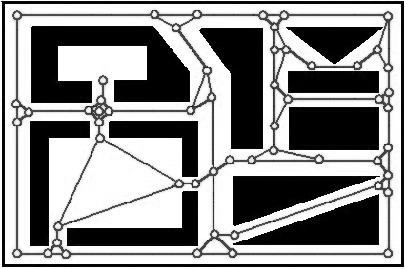
\includegraphics[width=0.75\columnwidth]{images/grafoExemplo.png}
	\caption*{Fonte: \citep{sampaiophd}}
	\label{fig:graphexample}
\end{figure}

Existem diversas métricas que podem compor o conjunto $M$. Um exemplo é o 
intervalo máximo que é definido como o maior intervalo entre visitas de todos os 
pontos de interesse \citep{sampaiophd}. Essa métrica é bastante utilizada em 
vários trabalhos da área \citep{6900280}, \cite{Pippin:2013:PBT:2480362.2480378}, 
\citep{Chevaleyre:2004:TAM:1018411.1019013}, \citep{6615158}. Outro exemplo, 
utilizado na literatura \citep{hernandez2013game}, é a ociosidade média, que 
consiste em calcular a média das ociosidades de cada ponto de interesse e depois 
tirar a média temporal desses valores.

Sendo assim, é possível concluir que o problema da Patrulha Multiagente é, 
fundamentalmente, um problema de otimização, onde é preciso escolher as ações 
dos agentes com a finalidade de minimizar (ou maximizar) uma dada métrica 
\citep{sampaiophd}.

A Computação Evolucionária engloba uma classe de algoritmos que realiza uma 
busca no espaço de soluções à procura daquela que seja ótima 
\citep{Luke2013Metaheuristics}. Esses algoritmos são baseados na Teoria da 
Evolução das Espécies proposta por Charles Darwin 
\footnote{http://en.wikipedia.org/wiki/Evolution}. Eles são chamados de \acp{ea}, 
pois buscam dentro de uma população, o indivíduo melhor adaptado. Numa analogia 
com a \ac{tmap}, um indivíduo seria uma sociedade de agentes que patrulha um 
território e as métricas de avaliação determinariam qual seria a solução melhor 
adaptada . Dessa forma, será mostrado no presente trabalho que \acp{ea} podem 
ser utilizados para resolver o problema a \ac{tmap}.

Apesar de possuir diversas soluções com diferentes abordagens para o problema 
\citep{Chevaleyre:2004:TAM:1018411.1019013}, 
\citep{Machado:2002:MPE:1765317.1765332}, \citep{Almeida:2004:AAI}, 
\citep{4209122}, \citep{hernandez2013game}, soluções que utilizam estratégias 
evolucionárias \citep{Luke2013Metaheuristics} são pouco encontradas na 
literatura \citep{4630897}, \citep{6900280} e, por tanto, serão o objeto de 
pesquisa do presente trabalho.

\section{Objetivos Gerais}

Motivado pelos problemas descritos acima, este trabalho tem como objetivo geral 
a proposição e o estudo de soluções para \ac{tmap} utilizando estratégias 
evolucionárias. Outro objetivo é comprovar a eficácia e avaliar a relevância de 
abordagens evolucionárias para o problema da patrulha através de experimentos 
empíricos e da comparação destas soluções com as obtidas através de abordagens 
já propostas na literatura e tidas como tradicionais.

\section{Objetivos Específicos}

Tendo em vista tais objetivos gerais, este projeto visa atingir os seguintes 
objetivos específicos:

\begin{itemize}
	\item Investigar estratégias evolucionárias e como elas podem ser aplicadas 
		ao problema da patrulha multiagente temporal;
	\item Desenvolver um(s) algoritmo(s) baseado(s) em estratégias 
		evolucionárias para a solução da \ac{tmap};
	\item Implementar os algoritmos desenvolvidos em um simulador capaz de 
		computar diversas métricas para uma dada solução da \ac{tmap}.
	\item Avaliar o desempenho do algoritmo no simulador e verificar eficácia
		da abordagem.
	\item Comparar empiricamente as soluções encontradas com aquelas já 
		publicadas na literatura.
\end{itemize}
\chapter{Trabalhos Relacionados}
\label{chp:background}

\section{Considerações Iniciais}

Um dos grandes obstáculos para o estudo do Problema da Patrulha Multiagente é a 
falta de concordância, dentre os pesquisadores, sobre nomenclatura, escopo e 
critérios de avaliação para as soluções propostas. Isso pode se dever ao fato do 
problema da patrulha estar presente em diferentes áreas como Inteligência 
Artificial, Sistemas Multiagentes e até Robótica \citep{sampaiophd}.

Há, na literatura, nomes diferentes para o problema da Patrulha Multiagente. Por 
exemplo, alguns autores \citep{hernandez2013game} chamam o problema de “patrulha 
multirobô” (ou Multi-Robot Patrolling, em inglês), outros \citep{6495145} se 
referem ao problema pelo nome de “patrulha temporal” (tradução de timed 
patrolling), já alguns pesquisadores \citep{Koenig:2001:TCA:375735.376463} 
utilizam o termo “cobertura de terreno” (terrain coverage, em inglês). No 
entanto, no decorrer do presente trabalho será utilizado o termo “Patrulha 
Multiagente”, pois ele é considerado mais apropriado por diversos pesquisadores 
\citep{6900280}, \citep{sampaiophd}, \citep{hernandez2013game} e \citep{6315145}.

O escopo é outro fator que varia entre os trabalhos. \citep{6615158}, por 
exemplo, faz uma análise do problema da patrulha onde o ambiente é dinâmico. 
Isto é, o grafo onde os agentes patrulham sofre alterações ao longo da execução 
do agente. Em um dado momento, o grafo pode ter vértices adicionados ou 
removidos. Já \citep{6900280} trabalham levando em conta que agentes podem ter 
velocidades diferentes. Os autores de \citep{Pippin:2013:PBT:2480362.2480378} 
levam em consideração que agentes podem agir com eficiência abaixo do esperado, 
isto é, o agente não pode ser confiado para realizar a tarefa que lhe foi 
passada sem falhas. Em \citep{4209122}, os autores consideram restrições de 
frequência, isso significa que cada nó tem a si designado um valor de frequência 
com a qual o nó \textbf{deve} ser visitado. Outro exemplo seria o trabalho feito 
em \citep{6495145} e \citep{Poulet:2012:b}, onde é feita uma análise do problema 
em uma configuração de sistema aberto. Sistemas abertos foram definidos em 
\citep{6040660} como aqueles agentes podem entrar e sair a qualquer momento da 
execução.

Na presente pesquisa, será utilizado o escopo para a Patrulha Multiagente 
doravante referido como "padrão", onde os agentes possuem eficiência idêntica, 
são confiáveis e não são retirados nem adicionados ao longo da patrulha. Quanto 
ao ambiente, o objeto de estudo deste trabalho compreende apenas ambientes que 
permanecem estáticos durante a execução dos agentes, e os pontos que devem ser 
patrulhados não possuem restrições de frequência.

Existem diversas métricas que podem ser utilizadas para medir a eficiência de 
cada solução para a \ac{tmap}. Diferentes pesquisadores utilizam métricas 
distintas. Em \citep{Machado:2002:MPE:1765317.1765332} foram propostas as 
métricas mais utilizadas para a \ac{tmap}. São elas: ociosidade instantânea do 
nó, ociosidade instantânea do grafo, ociosidade máxima e tempo de exploração. 
Depois deste trabalho, \citep{sampaiophd} propôs uma nova família de métricas 
baseadas nos intervalos entre visitas. As métricas utilizadas nos trabalhos mais 
recentes variam: \citep{6900280} e \citep{Pippin:2013:PBT:2480362.2480378} 
utilizam o intervalo máximo, já \citep{4209122} fazem uso da frequência mínima e 
\citep{hernandez2013game} compara as frequências mínimas.

Dessa forma, esta sessão visa, através de pesquisa bibliográfica, explorar os 
trabalhos relacionados para construir a base de conhecimento necessária para 
formular uma proposta compatível com o objetivo deste projeto. Serão discutidas 
as soluções para o problema da patrulha presentes na literatura 
classificando-as por seu escopo e métricas utilizadas na avaliação dos agentes.

\section{Levantamento Bibliográfico}

\subsection{Definições}

O problema da Patrulha é tipicamente modelado por um Grafo 
\citep{Rosen:2002:DMA:579402}. Segundo \citep{Almeida:2004:AAI}, isso se deve 
ao fato de que representar o problema por meio de um grafo faz com que o 
problema possa ser facilmente adaptado para um variedade de domínios desde 
terrenos até redes de computadores. \citep{sampaiophd} também considera que os 
grafos sejam o modelo preferencial para os ambientes da \ac{tmap}, pois são 
suficientemente poderosos para capturar as características do terreno mais 
relevantes para o problema. Essa capacidade do grafo pode ser confirmada por 
estudos que adotam grafos como modelo e posteriormente aplicam suas soluções em 
ambientes realistas contínuos \citep{Pippin:2013:PBT:2480362.2480378}.

Em \citep{Chevaleyre:2004:TAM:1018411.1019013}, o problema é matematicamente 
definido da seguinte forma:

O território onde os agentes patrulham é representado por um grafo $G(V,E)$, 
onde $V$ é o conjunto dos pontos de interesse que precisam ser patrulhados e 
$E$ representa o conjunto de arestas, $E \in V^{2}$, de $G$. Para toda aresta 
$(i,j) \in E$, onde $i,j \in V$, corresponde um peso $c_{i,j}$ representando a 
distância entre o vértices $i$ e $j$ em $G$. 

Nesse cenário, uma solução monoagente para o problema seria uma função 
$ \pi : \mathbb{N} \longrightarrow V$, tal que $ \pi(j)$ 
é o $j$-ésimo vértice visitado pelo agente, desde que 
$ \pi(j+1) = x $ se, e somente se, $ (\pi(j), x) \in E $. Analogamente, 
uma solução multiagente seria um conjunto $ \Pi = \{ \pi_{1} ... \pi_{r} \}$, 
onde $r$ é o número de agentes.

Dessa forma, o problema seria encontrar o conjunto $ \Pi $ que obtivesse os 
melhores resultados de acordo com um certo critério de avaliação.

Já \citep{sampaiophd} contribuiu com uma definição mais abrangente da \ac{tmap}. 
Ele aponta que uma instância da \ac{tmap} pode ser completamente definida pela 
seguinte tupla: 

$$ \langle E, P, S, s_{0}, A, I, M \rangle $$

O elemento $E$ representa o ambiente (do inglês, \textit{environment} onde estão 
os pontos de interesse a serem patrulhados, preferencialmente $E$ deve ser um 
grafo $G(V,E)$. E o elemento $P$ é o conjunto dos pontos de interesse do ambiente. 
No caso de um grafo, $P = V$.

$S$ é um elemento um pouco mais complexo, pois ele 
representa o conjunto de possíveis estados da sociedade de agentes. Cada estado 
dentro desse conjunto pode conter informações tais como, quantos agentes estão 
ativos, qual a posição atual de cada agente no ambiente $E$, o tempo decorrido 
desde o início da patrulha, orientação e energia de cada agente e 
características globais do conjunto de agentes. O estado inicial da sociedade é 
representado em $s_{0}$, ou seja, $s_{0} \in S$. Esta modelagem para o grupo de 
agentes permite ao modelo de \citep{sampaiophd} englobar diversas extensões para 
a \ac{tmap}, como por exemplo as citadas no \chapref{chp:introduction}.

O quinto elemento da tupla, $A$, é o conjunto de ações que alteram o estado da 
sociedade, $S$. Essas ações podem ser individuais, de cada agente, ou coletivas, 
da sociedade inteira. O autor afirma que $A$ deve conter, no mínimo, duas ações 
individuais definidas para cada agente: movimentação entre os pontos de $P$ e 
visitação aos elementos do conjunto.

$I$ representa o intervalo de medição, dentro do qual o desempenho dos agentes 
é mensurado através das métricas definidas no conjunto $M$, último elemento da 
tupla.

O problema da patrulha multiagente seria, então, definir um conjunto $A$ de 
ações a serem tomadas pelos agentes, que estão inicialmente no estado $s_{0}$, 
para minimizar as métricas presentes em $M$ durante o período de patrulha, $I$.

\subsection{Classificações para a \ac{tmap}}
\label{sec:classifytmap}

São notórios alguns trabalhos muito citados na literatura que visaram 
classificar as soluções para a \ac{tmap}.

Em \citep{Chevaleyre:2004:TAM:1018411.1019013}, as abordagens propostas até 
então foram classificadas em \textbf{cíclicas} (ou de ciclo único) e \textbf{
baseadas em particionamento}. As soluções de ciclo único são aquelas onde é 
calculado um ciclo que cobre todos os vértices do grafo, e então, os agentes são 
colocados para caminhar nesse ciclo indefinidamente. As abordagens baseadas em 
particionamento são aquelas onde o território a ser patrulhado é dividido em 
$r$ regiões, onde $r$ é o número de agentes. Os agentes devem, então, patrulhar 
dentro de suas respectivas regiões.

Já \citep{Machado:2002:MPE:1765317.1765332} fazem uma extensa classificação das 
arquiteturas de soluções para a \ac{tmap}. Eles dividem os agentes em: \textbf{
reativo} ou \textbf{cognitivo}; com comunicação \textbf{permitida} ou \textbf{
proibida}; com coordenação \textbf{central} ou \textbf{descentralizada}; com 
percepção \textbf{local} ou \textbf{global}; com tomada de decisão \textbf{
aleatória} ou \textbf{orientada a objetivo}. Os agentes reativos são aqueles que 
agem baseados apenas na sua percepção atual do território, enquanto que os 
agentes cognitivos podem perseguir um determinado objetivo. Enquanto os agentes 
cognitivos tem uma visão do grafo completo, os reativos só podem enxergar os nós 
adjacentes ao que eles se encontram. A comunicação se refere a possibilidade dos 
agentes trocarem informações. A percepção se refere ao quanto de informação o 
agente pode acessar sobre o ambiente ao seu redor e sobre os outros agentes. 
Finalmente, no esquema de coordenação centralizado, uma entidade central escolhe 
nó-objetivo de cada agente, enquanto que no esquema descentralizado, a 
coordenação emerge da interação entre os agentes.

As abordagens propostas na presente pesquisa podem ser classificadas como 
estratégias \textbf{baseadas em particionamento}, com agentes 
\textbf{cognitivos}, de comunicação \textbf{proibida}, com coordenação 
\textbf{centralizada}, de percepção \textbf{global}, e com tomada de decisão 
\textbf{orientada a objetivo}.

\subsection{Soluções já propostas}

\citep{Chevaleyre:2004:TAM:1018411.1019013} propuseram uma solução para a 
\ac{tmap} baseada no \ac{tsp}. Segundo os autores, a solução mais simples seria 
encontrar um ciclo que percorresse todos os pontos de interesse do terreno 
(de preferência sem repetição de pontos dentro do ciclo) e então fazer o agente 
percorrer esse ciclo indefinidamente. Esta estratégia corresponde a encontrar um 
ciclo que percorre todos os nós do grafo sem repeti-los, um Ciclo Hamiltoniano. 
O trabalho demonstra que para um único agente a solução ótima, para a métrica da 
ociosidade máxima, é esta estratégia cíclica baseada no \ac{tsp}. No entanto, 
o \ac{tsp} é conhecidamente um problema NP-Completo. Dessa forma, os autores 
propõem uma solução utilizando o algoritmo de Christofides 
\citep{christofides1976worst} para obter uma aproximação do \ac{tsp} em tempo 
polinomial. A pesquisa ainda aponta que, para o caso multiagente, a solução 
seria calcular o ciclo, posicionar os agentes com um certo intervalo entre um e 
outro e colocá-los para percorrer o ciclo indefinidamente. Os autores, no 
entanto, não estudam a aplicação dessa solução ao problema com outras métricas 
que não a da ociosidade máxima.

Posteriormente, \citep{Almeida:2004:AAI} realizam um estudo comparativo entre 
estratégias centralizadas e descentralizadas. Eles concluem que a solução 
proposta por \citep{Chevaleyre:2004:TAM:1018411.1019013} é a mais eficiente 
dentre as estudadas por eles. Os autores também chegam à conclusão de que as 
estratégias centralizadas estudadas, apesar de terem obtido resultados melhores 
nos experimentos, devem sofrer mais com problemas de escalabilidade a medida 
que o grafo cresce.

A partir das conclusões tiradas nesses estudos, \citep{4209122} propõem uma 
solução centralizada e cíclica, onde ao invés de utilizar o algoritmo de 
Christofides, se utiliza o método \textit{Spanning Tree Coverage}, introduzido 
em \citep{Gabriely:2001}, para gerar um Ciclo Hamiltoniano em um grafo com 
formato de \textit{grid}. Assim como a solução de 
\citep{Chevaleyre:2004:TAM:1018411.1019013}, após o ciclo ser calculado, os 
vários agentes são posicionados no grafo e colocados para percorrer o ciclo 
indefinidamente.

Além dessas soluções de ciclo único, também foram propostas, na literatura, 
soluções baseadas em particionamento. Os autores 
\citep{Pippin:2013:PBT:2480362.2480378} propõem uma solução, onde, na 
inicialização, os nós do grafo são particionados entre os agentes e esses 
calculam um ciclo fechado (\textit{closed cycle}) dentro da respectiva partição. 
Uma entidade de monitoramento central fica responsável por verificar, ao longo 
da execução, a performance dos agentes para a métrica de intervalo máximo entre 
visitas e identificar agentes que estejam com baixo desempenho. Então, alguns 
nós do agente de baixo rendimento são oferecidos aos outros agentes e 
redesignados através de um protocolo baseado em leilão.

Visando a escalabilidade apontada por \citep{Almeida:2004:AAI}, foram propostas 
diversas soluções descentralizadas. Dentre elas, destacam-se as baseadas em 
colônias de formigas \citep{Koenig:2001:TCA:375735.376463}, 
\citep{Elor:2010:AMC:1884958.1884970}, \citep{6615158}. Nessas soluções, os 
agentes não possuem uma visão completa do grafo, mas apenas das suas 
vizinhanças. A coordenação dos agentes é emergente 
\citep{Machado:2002:MPE:1765317.1765332}, pois cada agente pode deixar marcações 
em nós do grafo que podem ser sentidas pelos outros agentes. Ao comparar as 
soluções centralizadas com as descentralizadas, \citep{Almeida:2004:AAI} 
encontra resultados melhores nas centralizadas.

Apesar de serem amplamente utilizados na literatura para resolver problemas de 
otimização, os Algoritmos Evolucionários \citep{Luke2013Metaheuristics} foram 
pouco utilizados no problema da Patrulha. \citep{4630897} propõe uma solução 
híbrida composta de dois passos: no primeiro, um algoritmo genético para 
posicionar os agentes o mais distante possível dentro do território, e então, 
utiliza \ac{aco} para calcular partições no grafo por onde os agentes irão 
patrulhar durante a execução. Dessa forma, pode-se constatar que o algoritmo 
evolucionário não está sendo usado para resolver o problema da patrulha em si, 
mas para encontrar os $r$ nós mais distantes uns dos outros dentro do grafo, 
onde $r$ é o número de agentes.

\section{Considerações Finais}

Uma vez apresentados, neste capítulo, os conceitos básicos dos trabalhos 
relacionados, é possível fazer algumas observações sobre tendências dentre as 
publicações. Há uma predileção pela Simulação como método de comparação e de 
demonstração de soluções. É possível também perceber que muitos trabalhos 
utilizam as métricas propostas por \citep{Machado:2002:MPE:1765317.1765332} e 
\citep{sampaiophd}.


Percebe-se que falta à literatura um trabalho que investigue uma solução para a 
\ac{tmap} utilizando algoritmos evolucionários, tais como as \acp{es} e os 
\acp{ga}.

A \tabref{tbl:comp_background} resume as soluções apresentadas nesta sessão de 
acordo com o escopo do problema, o método de demonstração das soluções e as 
métricas utilizadas.

\begin{table}[tp]
	\centering
	\caption{Resumo dos trabalhos relacionados}
	\label{tbl:comp_background}
	\begin{tabularx}{\linewidth}{|X|X|X|X|}
		\hline
		\textbf{Trabalho} & \textbf{Escopo} & \textbf{Método} & \textbf{Métrica(s)} \\
		\hline
		\citep{Machado:2002:MPE:1765317.1765332} & Patrulha Multiagente "Padrão" & Simulação & Ociosidade instantânea do nó, ociosidade instantânea do grafo, ociosidade do grafo, ociosidade máxima e tempo de exploração \\
		\hline
		\citep{Chevaleyre:2004:TAM:1018411.1019013} & Patrulha Multiagente "Padrão" & Análise Matemática & Pior ociosidade (\textit{worst idleness}) \\
		\hline
		\citep{Almeida:2004:AAI} & Patrulha Multiagente "Padrão" & Simulação & Ociosidade do grafo, Ociosidade média normalizada e Desvio padrão da ociosidade média \\
		\hline
		\citep{4209122} & Patrulha Multiagente com restrição de frequência & Análise Matemática & Frequência máxima uniforme \\
		\hline
		\citep{4630897} & Patrulha Multiagente "Padrão" & Simulação & Ociosidade Máxima \\
		\hline
		\citep{6495145} & Patrulha Multiagente como um sistema aberto & Simulação & Intervalo médio entre visitas, Intervalo quadrático médio, tempo de estabilização e amplitude das variações \\
		\hline
		\citep{Pippin:2013:PBT:2480362.2480378} & Patrulha Multiagente com agentes que possuem performances distintas & Simulação e Experimentação com robôs reais & Intervalo Máximo entre visitas \\
		\hline
		\citep{6615158} & Patrulha Multiagente em ambientes dinâmicos & Simulação & Intervalo Máximo entre visitas \\
		\hline
		\citep{hernandez2013game} & Patrulha Multiagente "Padrão" & Simulação & Ociosidade total \\
		\hline
	\end{tabularx}
	\caption*{Fonte: O autor}
\end{table}
\chapter{Algoritmos Evolucionários}

Sendo o objetivo do presente trabalho apresentar abordagens evolucionárias para 
a \ac{tmap}, este capítulo tem como finalidade apresentar ao leitor alguns 
conceitos e terminologias da área da Computação Evolucionária, para que ele 
esteja familiarizado antes do capítulo sobre a aplicação de algoritmos 
evolucionários no contexto da \ac{tmap}. Este capítulo também vai apresentar os 
algoritmos que foram utilizados na pesquisa.

Segundo \citep{Back:1993:OEA:1326623.1326625}, várias pesquisas mostraram, ao 
longo de três séculos, que modelar o processo de busca de forma similar à evolução 
pelo qual os seres vivos passaram pode render algoritmos robustos, mesmo que 
estes modelos sejam apenas representações imperfeitas do verdadeiro processo 
biológico. O resultado desses modelos são chamados de Algoritmos Evolutivos ou 
Evolucionários. Essa busca pode ser aplicada para encontrar não apenas uma 
solução qualquer, mas aquela que minimize ou maximize uma dada métrica. Dessa 
forma, algoritmos evolucionários podem (e são) utilizados em problemas de 
otimização.

Tais algoritmos são baseados no processo de aprendizado coletivo pelo qual passa 
uma população de indivíduos. Cada indivíduo representa uma solução para um 
problema, ou um ponto no espaço de possíveis soluções. O ambiente fornece 
informações qualitativas sobre cada indivíduo. Essa informação pode ser 
interpretada como a aptidão do indivíduo no ambiente determinado. Na 
analogia com algoritmos, essa é a medida de avaliação de uma solução 
\citep{Back:1993:OEA:1326623.1326625}.

Um algoritmo evolucionário funciona, genericamente, da seguinte forma: uma 
população inicial é arbitrariamente inicializada; esse indivíduos têm sua 
adaptação ao ambiente medida; eles são, posteriormente, recombinados para formar 
uma nova população, podendo também sofrer mutação; finalmente, um subconjunto 
dessas populações (antiga e nova, pais e filhos) é selecionado de alguma forma 
definida pelo algoritmo e se torna a população da próxima geração. Esse ciclo 
se repete tipicamente até que parem de surgir melhores indivíduos que aqueles já 
presentes na população, evento chamado de convergência do algoritmo 
\citep{Back:1993:OEA:1326623.1326625}.

A população inicial pode ser criada de forma aleatória, ou pode-se utilizar 
conhecimentos sobre o problema para inicializar uma população onde os indivíduos 
estão em uma região "boa" (de acordo com a métrica) do espaço de soluções 
\citep{Luke2013Metaheuristics}.

O Pseudocódigo~\ref{EAGeneric} abaixo exemplifica de forma genérica um algoritmo 
evolucionário.

\begin{algorithm}                      % enter the algorithm environment
	\caption{Algoritmo Evolucionário Genérico}          % give the algorithm a caption
	\label{EAGeneric}                           % and a label for \ref{} commands later in the document
	\begin{algorithmic}                    % enter the algorithmic environment
		\Procedure{EA}{}
		\State $P \gets $ Constrói-População-Inicial
		\Repeat
			\State $P^{\prime} \gets $ Recombina($P$)
			\State $P^{\prime \prime} \gets $ Aplica-Mutação($P^{\prime}$)
			\State $P \gets $ Seleciona($P^{\prime \prime}$)
		\Until{não termos mais tempo}
		\EndProcedure
	\end{algorithmic}
\end{algorithm}

A \tabref{tbl:evo_dict} revisa alguns dos termos comumente utilizados nos 
\acp{ea}.

No restante do presente capítulo, serão apresentados os algoritmos utilizados 
nesta pesquisa, as Estratégias Evolucionárias e os Algoritmos Genéticos. Cada 
um desses possui duas variações que foram aplicadas na pesquisa: 
$( \mu,\lambda )$ ou $( \mu + \lambda )$ e Geracional ou Estado Estável 
(em inglês, \textit{steady state}), respectivamente.

\begin{table}[tp]
	\centering
	\caption{Termos comuns na Computação Evolucionária}
	\label{tbl:evo_dict}
	\begin{tabularx}{\linewidth}{|X|X|}
		\hline
		\textbf{Termo} & \textbf{Significado} \\
		\hline
		Indivíduo & Uma solução candidata \\
		\hline
		Filha e Pai & Uma solução Filha é uma cópia alterada de uma solução Pai \\
		\hline
		População & Um conjunto de soluções candidatas \\
		\hline
		Aptidão & Qualidade de um indivíduo (Solução) \\
		\hline
		Seleção & Coletar indivíduos baseados na sua aptidão \\
		\hline
		Mutação & Realização de pequenas alterações em indivíduos. Também chamada de reprodução assexuada \\
		\hline
		Recombinação (em inglês, \textit{crossover}) & Uma forma de alteração especial que recebe como parâmetro duas soluções pais e (normalmente) produz duas soluções filhas \\
		\hline
		Reprodução & O ato de produzir uma ou mais soluções filhas a partir de uma solução pai \\
		\hline
		Geração & Um ciclo de medida de aptidão ou de reprodução de uma população \\
		\hline
%		\citep{Machado:2002:MPE:1765317.1765332} & Patrulha Multiagente "Padrão" & Simulação & Ociosidade instantânea do nó, ociosidade instantânea do grafo, ociosidade do grafo, ociosidade máxima e tempo de exploração \\
%		\hline
	\end{tabularx}
	\caption*{Fonte: Adaptado de \citep{Luke2013Metaheuristics}}
\end{table}

\section{Estratégias Evolucionárias}

As duas estratégias evolucionárias usadas no presente trabalho se diferem pela 
forma como fazem a composição entre a população de pais e a população de filhos 
para construir a nova geração, que será utilizada na iteração seguinte do 
algoritmo.

A primeira \ac{es} é conhecida como $( \mu, \lambda )$. Tipicamente, começa-se 
com uma população de $\lambda$ indivíduos gerados de forma arbitrária. Nessa 
\ac{es}, o $\mu$ representa o número de pais cujos filhos serão usados para compor 
a próxima população que também deve ter $\lambda$ indivíduos no total. Note que 
$\lambda$ tem que ser um múltiplo de $\mu$. Então, os $\mu$ indivíduos mais 
aptos são escolhidos, processo chamado de Seleção por Truncamento (em inglês, 
\textit{Truncate Selection}). Os indivíduos selecionados sofrem mutação para 
gerar $ \lambda / \mu $ filhos. O que acarretará em uma nova população de 
$\lambda$ indivíduos que será a geração utilizada na próxima iteração do 
algoritmo \citep{Luke2013Metaheuristics}.

O Pseudocódigo~\ref{mu_lambda_es}, adaptado de \citep{Luke2013Metaheuristics}, 
exemplifica a Estratégia Evolucionária $( \mu, \lambda )$.

\begin{algorithm}                      % enter the algorithm environment
	\caption{Estratégia Evolucionária $( \mu, \lambda )$}          % give the algorithm a caption
	\label{mu_lambda_es}                           % and a label for \ref{} commands later in the document
	\begin{algorithmic}                    % enter the algorithmic environment
		\Procedure{$ \mu\_\lambda $\_ES}{$ \mu, \lambda $}
		\State $P \gets \{\} $
		\For{$1 ... \lambda$}
			\State $p \gets$ \{novo indivíduo gerado de forma arbitrária\}
			\State CalculaAptidão($p$)
			\State $P \gets P \ \cup $ \{$p$\} 
		\EndFor
		\State $Melhor \gets$ nulo
		\Repeat
			\State Ordena($P$) \Comment{Ordena a população de acordo com a aptidão}
			\State $Q \gets P_{1...\mu}$ \Comment{Inicia $Q$ com os $\mu$ indivíduos mais aptos}
			\State $P \gets \{\}$
			\For{$Q_{j} \in Q$}
				\For{$1... \lambda / \mu$}
					\State $P \gets P \ \cup $ \{Aplica-Mutação($Q_{j}$)\}
				\EndFor
			\EndFor
			\For{$P_{i} \in P$}
				\State CalculaAptidão($P_{i}$)
				\If{$Melhor = $ nulo \textbf{ou} Aptidão($P_{i}$) > Aptidão($Melhor$)}
					\State $Melhor \gets P_{i}$
				\EndIf
			\EndFor
		\Until{não termos mais tempo}
		\State \textbf{return} $Melhor$
		\EndProcedure
	\end{algorithmic}
\end{algorithm}

A segunda \ac{es} utilizada nesta pesquisa é chamada de $( \mu + \lambda)$. 
Enquanto que na estratégia $( \mu, \lambda )$ cada pai é substituído pelos seus 
$ \lambda / \mu $ filhos, na estratégia $( \mu + \lambda )$, os $\mu$ pais 
permanecem para competir com seus $ \lambda$ filhos na iteração seguinte. 
\citep{Luke2013Metaheuristics} aponta que isso geralmente faz com que a 
estratégia $( \mu + \lambda )$ explore mais os ótimos locais em comparação com 
a estratégia $( \mu, \lambda )$, já que um pai suficientemente apto pode fazer 
com que a \ac{es} fique "presa" em seus descendentes imediatos, causando uma 
convergência das populações para o ótimo local ao redor do pai.

O Pseudocódigo~\ref{mu+lambda_es}, também adaptado de 
\citep{Luke2013Metaheuristics}, ilustra a Estratégia Evolucionária 
$( \mu + \lambda )$.

\begin{algorithm}                      % enter the algorithm environment
	\caption{Estratégia Evolucionária $( \mu + \lambda )$}          % give the algorithm a caption
	\label{mu+lambda_es}                           % and a label for \ref{} commands later in the document
	\begin{algorithmic}                    % enter the algorithmic environment
		\Procedure{$ \mu+\lambda $\_ES}{$ \mu, \lambda $}
		\State $P \gets \{\} $
		\For{$1 ... \lambda$}
			\State $p \gets$ \{novo indivíduo gerado de forma arbitrária\}
			\State CalculaAptidão($p$)
			\State $P \gets P \ \cup $ \{$p$\} 
		\EndFor
			\State $Melhor \gets$ nulo
		\Repeat
			\State Ordena($P$) \Comment{Ordena a população de acordo com a aptidão}
			\State $Q \gets P_{1...\mu}$ \Comment{Inicia $Q$ com os $\mu$ indivíduos mais aptos}
			\State $P \gets Q$ \Comment{A diferença está aqui}
			\For{$Q_{j} \in Q$}
				\For{$1... \lambda / \mu$}
					\State $P \gets P \ \cup $ \{Aplica-Mutação($Q_{j}$)\}
				\EndFor
			\EndFor
			\For{$P_{i} \in P$}
				\State CalculaAptidão($P_{i}$)
				\If{$Melhor = $ nulo \textbf{ou} Aptidão($P_{i}$) > Aptidão($Melhor$)}
					\State $Melhor \gets P_{i}$
				\EndIf
			\EndFor
		\Until{não termos mais tempo}
		\State \textbf{return} $Melhor$
		\EndProcedure
	\end{algorithmic}
\end{algorithm}

É importante notar que as Estratégias Evolucionárias não utilizam a recombinação 
para gerar novos indivíduos. Para isso, elas utilizam apenas a Mutação cuja 
implementação depende do tipo de dados envolvido no problema que está sendo 
estudado. No próximo capítulo, serão propostos alguns operadores de Mutação para 
a \ac{tmap}, que irão agir sobre caminhos e ciclos de um grafo. Também será 
tratado, no próximo capítulo, como foram implementadas as funções de gerar 
indivíduos e calcular suas aptidões dentro do contexto da \ac{tmap}.

\section{Algoritmos Genéticos}

Os Algoritmos Genéticos são similares às \acp{es}: o seu \textit{loop} principal 
consiste em selecionar indivíduos da polução de acordo com as respectivas 
aptidões, reproduzir os indivíduos selecionados e iterar sobre a nova população 
para calcular as novas aptidões \citep{Luke2013Metaheuristics}.

No entanto, eles são diferentes na forma como selecionam e reproduzem os 
indivíduos. Enquanto que nas Estratégias Evolucionárias, todos os pais são 
selecionados simultaneamente e passam por mutação em seguida, os Algoritmos 
Genéticos selecionam os pais e geram filhos ao poucos até que se tenha uma 
população de filhos suficiente. A reprodução em si também é bem diferente das 
\acp{es}: nos Algoritmos Genéticos, inicia-se com uma população de filhos vazia. 
O Algoritmo então seleciona dois pais de forma arbitrária, recombina esses pais 
em dois novos indivíduos filhos e então faz a mutação deles. Esses dois novos 
indivíduos são adicionados à população. Esse processo se repete até que a 
população de filhos esteja completamente preenchida 
\citep{Luke2013Metaheuristics}.

O pseudocódigo~\ref{GenAlg}, adaptado de \citep{Luke2013Metaheuristics}, deve 
ajudar o leitor a compreender o algoritmo.

\begin{algorithm}                      % enter the algorithm environment
	\caption{Algoritmo Genético}          % give the algorithm a caption
	\label{GenAlg}                           % and a label for \ref{} commands later in the document
	\begin{algorithmic}                    % enter the algorithmic environment
		\Procedure{AlgoritmoGenetico}{$tamanhoPopulação$}
		\State $P \gets \{\} $
		\For{$1 ...\ tamanhoPopulação$}
			\State $p \gets$ \{novo indivíduo gerado de forma arbitrária\}
			\State CalculaAptidão($p$)
			\State $P \gets P \ \cup $ \{$p$\} 
		\EndFor
		\State $Melhor \gets$ nulo
		\Repeat
			\State $Q \gets \{\}$
			\For{$1 ...\ tamanhoPopulação / 2$}
				\State $Pai_{a} \gets $ Seleciona($P$)
				\State $Pai_{b} \gets $ Seleciona($P$)
				\State $Filho_{a},\ Filho_{b} \gets $ Recombina($Pai_{a}$, $Pai_{b}$)
				\State $Q \gets Q\ \cup $ \{Aplica-Mutação($Filho_{a}$), Aplica-Mutação($Filho_{b}$)\}
			\EndFor
			\State $P \gets Q$
			\For{$P_{i} \in P$}
				\State CalculaAptidão($P_{i}$)
				\If{$Melhor = $ nulo \textbf{ou} Aptidão($P_{i}$) > Aptidão($Melhor$)}
					\State $Melhor \gets P_{i}$
				\EndIf
			\EndFor
		\Until{não termos mais tempo}
		\State \textbf{return} $Melhor$
		\EndProcedure
	\end{algorithmic}
\end{algorithm}

Esta é a forma tradicional como o Algoritmo Genético é apresentado nos livros 
textos \citep{Luke2013Metaheuristics}, também conhecido como Algoritmo Genético 
Geracional. No entanto, existem outras variações, como por exemplo, o Algoritmo 
Genético de Estado Estável, do inglês, \textit{Steady State Genetic Algorithm}.
O \ac{ga} Geracional é assim conhecido pois nele a população é completamente 
atualizada de uma vez. O \ac{ga} de Estado Estável, por sua vez, introduz um 
ou dois filhos, obtidos através de recombinação e mutação, diretamente na 
população de indivíduos (matando outros indivíduos para abrir espaço) e segue 
para a próxima geração.

Dessa forma, assim como a \ac{es} $( \mu + \lambda )$, os indivíduos pais se 
mantém na população e disputam com os filhos nas gerações seguintes. Por isso, 
este algoritmo pode sofrer do mesmo problema e ficar "preso" a ótimos locais ao 
redor dos pais \citep{Luke2013Metaheuristics}.

O pseudocódigo~\ref{GenAlgSteady}, adaptado de \citep{Luke2013Metaheuristics}, detalha 
as características do Algoritmo Genético de Estado Estável.

\begin{algorithm}                      % enter the algorithm environment
	\caption{Algoritmo Genético de Estado Estável}          % give the algorithm a caption
	\label{GenAlgSteady}                           % and a label for \ref{} commands later in the document
	\begin{algorithmic}                   % enter the algorithmic environment
		\Procedure{AlgoritmoGeneticoEstadoEstavel}{$tamanhoPopulação$}
		\State $P \gets \{\} $
		\For{$1 ...\ tamanhoPopulação$}
			\State $P \gets P \ \cup $ \{novo indivíduo gerado de forma arbitrária\} 
		\EndFor
		\For{$P_{i} \in P$}
			\State CalculaAptidão($P_{i}$)
			\If{$Melhor = $ nulo \textbf{ou} Aptidão($P_{i}$) > Aptidão($Melhor$)}
				\State $Melhor \gets P_{i}$
			\EndIf
		\EndFor
		\Repeat
			\State $Pai_{a} \gets $ Seleciona($P$)
			\State $Pai_{b} \gets $ Seleciona($P$)
			\State $Filho_{a},\ Filho_{b} \gets $ Recombina($Pai_{a}$, $Pai_{b}$)
			\State $Filho_{a} \gets $ Aplica-Mutação($Filho_{a}$)
			\State $Filho_{b} \gets $ Aplica-Mutação($Filho_{b}$)
			\State CalculaAptidão($Filho_{a}$)
			\If{Aptidão($Filho_{a}$) > Aptidão($Melhor$)}
				\State $Melhor \gets Filho_{a}$
			\EndIf
			\State CalculaAptidão($Filho_{b}$)
			\If{Aptidão($Filho_{b}$) > Aptidão($Melhor$)}
				\State $Melhor \gets Filho_{b}$
			\EndIf
			\State $p_{c} \gets $ SelecionaParaMorrer($P$) \Comment{Seleciona um indivíduo para remover da população}
			\State $p_{d} \gets $ SelecionaParaMorrer($P$) \Comment{$p_{c} \neq p_{d}$}
			\State $P \gets P\ -\ \{p_{c},p_{d}\}$
			\State $P \gets P\ \cup\ \{Filho_{a},\ Filho_{b}\}$
		\Until{não termos mais tempo}
		\State \textbf{return} $Melhor$
		\EndProcedure
	\end{algorithmic}
\end{algorithm}

No próximo capítulo, serão explorados as aplicações dos algoritmos acima 
apresentados para a \ac{tmap}. Serão propostos operadores de mutação e de 
recombinação que possam ser aplicados ao modelo utilizado, além de um método 
para calcular a aptidão de um indivíduo. No entanto, pode-se, ainda neste 
capítulo, tratar de um operador utilizado nos algoritmos genéticos que é 
definido sem interferência do problema ou da estrutura de dados no qual ele 
está modelado. Os operadores de Seleção podem ser descritos para uma população 
qualquer de indivíduos modelados de forma arbitrária.

Na presente pesquisa, foi utilizado o operador de mutação comumente chamado de 
Torneio (do inglês, \textit{Tournament}) \citep{Luke2013Metaheuristics}. Ele 
consiste em coletar, da população, $t$ indivíduos de forma aleatória. Destes, 
o algoritmo retorna apenas o indivíduo mais apto. Segue o pseudocódigo para 
ilustrar esse operador \citep{Luke2013Metaheuristics}.

\begin{algorithm}                      % enter the algorithm environment
	\caption{Torneio}          % give the algorithm a caption
	\label{torneio}                           % and a label for \ref{} commands later in the document
	\begin{algorithmic}                    % enter the algorithmic environment
		\Procedure{Torneiro}{$P, t$}
		\State $Melhor \gets $ indivíduo escolhido aleatoriamente de $P$ \Comment{De forma que não possa ser escolhido uma segunda vez}
		\For{$i$ de $2 ... t$}
			\State $Proximo \gets $ indivíduo escolhido aleatoriamente de $P$
			\If{Aptidão($Proximo$) $>$ Aptidão($Melhor$)}
				\State $Melhor \gets Proximo$
			\EndIf
		\EndFor
		\State \textbf{return} $Melhor$
		\EndProcedure
	\end{algorithmic}
\end{algorithm}
\chapter{Conclusão}
\label{conclusao_final}

Como mostrado neste documento, a Patrulha Multiagente Temporal tem sido o objeto 
de estudo de diversas pesquisas, pois trata-se de um problema difícil e 
desafiador da área de Inteligência Artificial e Sistemas Multiagente com 
diversas aplicações em cenários reais.

No entanto, também foi verificado, que apesar de ser essencialmente um problema 
de otimização, não haviam sido estudadas aplicações diretas de algoritmos 
evolucionários para encontrar soluções para a \ac{tmap}.

Assim, após revisar quatro algoritmos bastante utilizados na Computação 
Evolucionária, a presente pesquisa apresentou dez operadores que podem ser 
combinados com esses algoritmos de diferentes maneiras para formar dezenas de 
heurísticas evolucionárias distintas capazes de resolver a \ac{tmap}.

Além disso, foi demonstrado através de experimentos que os operadores aqui 
apresentados são eficazes em produzir boas soluções. Também foram apontados 
os operadores e suas combinações que proporcionaram as melhores soluções. 
E foi mostrado empiricamente que a qualidade das soluções encontradas por estas 
heurísticas evolucionárias são comparáveis com a de algumas das melhores 
abordagens apresentadas na literatura.

Já que as soluções propostas visam criar uma sociedade de agentes onde cada um 
fica responsável por uma partição do grafo, este trabalho corrobora com as 
conclusões de \citep{1373634}: especializar agentes em sub-regiões do grafo 
produz bons resultados na \ac{tmap}.

\section{Trabalhos Futuros}

Este capítulo conclui o trabalho com algumas atividades que poderiam ter sido 
desenvolvidas, não fosse o período de tempo curto disponibilizado para sua 
conclusão.

Foi observado durante os experimentos que os operadores de mutação geravam 
indivíduos novos diferentes o bastante dos pais para permitir encontrar novas 
soluções e evoluir a população. No entanto, foi possível perceber ao longo dos 
experimentos realizados que esses operadores geravam indivíduos muito próximos 
uns dos outros. Fica como trabalho futuro investigar operadores de mutação mais 
exploratórios, que levem a uma diversidade maior da população, para que a busca 
no espaço de soluções seja mais global e não fique estagnada ao redor de mínimos 
locais. Também seria possível adicionar probabilidades para a execução de cada 
operação envolvida na mutação dos indivíduos: por exemplo, poderia executar o 
operador \textit{Melhorar} ao final da mutação apenas com uma probabilidade $x$.

Outra contribuição para o futuro seria investigar o impacto de outros operadores 
de seleção nos algoritmos genéticos. Principalmente o algoritmo genético de 
estado estável que utiliza duas seleções distintas: uma para escolher os 
indivíduos que deverão sofrer recombinação e outra para escolher os indivíduos 
da geração mais velha que serão eliminados para dar lugar às novas soluções 
recém-descobertas por meio da mutação e recombinação. Na presente pesquisa, 
esta última seleção foi configurada como Seleção da Pior Aptidão, ou seja, os 
indivíduos menos aptos seriam escolhidos para dar lugar. Uma outra seleção 
que pudesse eventualmente selecionar indivíduos bastante aptos, poderia fazer 
com que a busca do algoritmo genético de estado estável escapasse de mínimos 
locais em volta desses.

Nos experimentos de \textit{tuning}, os operadores puramente aleatórios, como 
por exemplo, o \textit{Random Centering} e \textit{Random Partitioning}, tiveram 
um desempenho bem abaixo dos seus concorrentes. Seria de grande valia investigar 
se, dado mais tempo de execução para os algoritmos evolucionários, os operadores 
puramente aleatórios poderiam ser vantajosos, proporcionando uma busca mais 
global para os algoritmos. Seria possível, por exemplo, executar esses 
algoritmos até que não houvesse melhora nos indivíduos de uma geração para a 
seguinte.

Seria interessante ainda realizar mais experimentos: utilizar uma quantidade 
maior e mais diversificada (topologicamente) de grafos, podendo também variar 
o tamanho da sociedade de agentes em intervalos mais curtos. Uma vez que mais 
dados seriam gerados, poderiam ser realizada uma análise estatística dos 
resultados a procura de maiores informações sobre as abordagens evolucionárias.

% References

\begin{references}
  \bibliography{references}
\end{references}

% Appendix

\theappendix
\chapter{Mapping Study's Instruments}
\label{ap:mapping-study}

\begin{table}[!htp]
	\centering
	\caption{List of conferences on which the searches were performed.}
	\label{tbl:conferences_list}
	\rowcolors{2}{lightgray!30}{white}
	\resizebox{\columnwidth}{!}{
	\begin{tabular}{ll}
	\toprule
	\textbf{Acronym} & \textbf{Conference} \\
	\toprule
	APSEC & Asia Pacific Software Engineering Conference \\
	ASE   & IEEE/ACM International Conference on Automated Software Engineering \\
	CSMR  & European Conference on Software Maintenance and Reengineering \\
	ESEC  & European Software Engineering Conference \\
	ESEM  & International Symposium on Empirical Software Management and Measurement \\
	ICSE  & International Conference on Software Engineering \\
	ICSM  & International Conference on Software Maintenance \\
	ICST & International Conference on Software Testing \\
	InfoVis & IEEE Information Visualization Conference \\
	KDD   & ACM SIGKDD International Conference on Knowledge Discovery and Data Mining \\
	MSR   & Working Conference on Mining Software Repositories \\
	OOPSLA & Object-Oriented Programming, Systems, Languages and Applications \\
	QSIC  & International Conference On Quality Software \\
	SAC & ACM Symposium on Applied Computing \\
	SEAA & EUROMICRO Conference on Software Engineering and Advanced Applications\\
	SEDE & 19th International Conference on Software Engineering and Data Engineering \\
	SEKE  & International Conference on Software Engineering and Knowledge Engineering \\
	\bottomrule
	\end{tabular}
	}
\end{table}

\begin{table}[htp]
	\caption{List of journals in which the searches were performed.}
	\label{tbl:journals_list}
	\centering
	\rowcolors{2}{lightgray!30}{white}
	\begin{tabular}{l}
	\toprule
	\textbf{Journal title} \\
	\toprule
	ACM Transactions on Software Engineering and Methodology \\
	Automated Software Engineering \\
	Elsevier Information and Software Technology \\
	Elsevier Journal of Systems and Software \\
	Empirical Software Engineering \\
	IEEE Software \\
	IEEE Computer \\
	IEEE Transactions on Software Engineering \\
	International Journal of Software Engineering and Knowledge Engineering \\
	Journal of Software: Evolution and Process \\
	Software Quality Journal \\
	Journal of Software \\
	Software Practice and Experience Journal \\
	\bottomrule
	\end{tabular}
\end{table}

\begin{table}[h]
\centering
\footnotesize
 \rowcolors{2}{lightgray!30}{white}
\caption{Search string per Search Engine.}
\label{tbl:stringengine}
\begin{tabular}{p{.15\textwidth}p{.8\textwidth}}
\toprule
\textbf{Search Engine} & \textbf{Search String}\\
\toprule
   	 	Google Scholar &  bug report OR track OR triage ``change
   	 	request'' issue track OR request OR software OR ``modification request'' OR
   	 	``defect track'' OR ``software issue''  repositories maintenance evolution\\

   	 	ACM Portal & Abstract: "bug report" or Abstract:"change request"
   	 	or Abstract:"bug track" or Abstract:"issue track" or  Abstract:"defect
   	 	track" or Abstract:"bug triage" or Abstract: "software issue" or Abstract: "issue request"
   	 	or Abstract: "modification request") and  (Abstract:software or
   	 	Abstract:maintenance or Abstract:repositories or Abstract:repository \\

   	 	IEEExplorer (1) & (((((((((("Abstract": "bug report") OR
   	 	"Abstract":"change request") OR "Abstract":"bug track") OR "Abstract":"software issue") OR "Abstract":"issue request") OR
        "Abstract":"modification request") OR "Abstract":"issue track") OR
	    "Abstract":"defect track") OR "Abstract":"bug triage") AND
	    "Abstract":software)\\

         IEEExplorer (2) & (((((((((("Abstract": "bug report") OR
         "Abstract":"change request") OR "Abstract":"bug track") OR "Abstract":"software issue") OR
         "Abstract":"issue request") OR "Abstract":"modification request") OR
         "Abstract":"issue track") OR "Abstract":"defect track") OR
         "Abstract":"bug triage") AND "Abstract":maintenance)\\

         IEEExplorer (3) & (((((((((("Abstract": "bug report") OR
         "Abstract":"change request") OR "Abstract":"bug track") OR "Abstract":"software issue") OR
         "Abstract":"issue request") OR "Abstract":"modification request") OR
         "Abstract":"issue track") OR "Abstract":"defect track") OR
         "Abstract":"bug triage") AND "Abstract":repositories)\\

         IEEExplorer & (((((((((("Abstract": "bug report") OR
         "Abstract":"change request") OR "Abstract":"bug track") OR "Abstract":"software issue") OR
         "Abstract":"issue request") OR "Abstract":"modification request") OR
         "Abstract":"issue track") OR "Abstract":"defect track") OR
         "Abstract":"bug triage") AND "Abstract": repository)\\

         Citeseer Library & (abstract: "bug report" OR abstract:"change request" OR abstract:"bug track" OR abstract:"issue track" OR
	     abstract:"defect track" OR abstract:"bug triage" OR abstract: "software
	     issue" OR abstract: "issue request" OR abstract: "modification request")
	     AND (abstract:software OR abstract:maintenance OR abstract:repositories OR
	     abstract:repository)\\

	     Elsevier & ("bug report" OR "change
	     request" OR "bug track" OR "issue track" OR "defect track" OR "bug triage" OR "software issue" OR  "issue request" OR
	    "modification request") AND (software OR maintenance OR repositories OR
	    repository)\\

	    Scirus & ("bug report" OR "change request" OR "bug track" OR "issue track" OR  "defect track" OR "bug triage" OR
        "software issue" OR  "issue request" OR "modification request") AND
	    (software maintenance OR repositories OR repository) ANDNOT (medical OR
	    aerospace)\\

	    ScienceDirect & ("bug report" OR "change request" OR "bug track"
	     OR "issue track" OR "defect track" OR "bug triage" OR "issue request" OR
	     "modification request") AND LIMIT-TO(topics, "soft ware")\\

	     Scopus & ("bug report" OR "change request" OR "bug track" OR
	     "issue track" OR  "defect track" OR "bug triage" OR "software issue" OR
	     "issue request" OR "modification request") AND (software maintenance OR
	     repositories OR repository)\\

	     Wiley & ("bug report" OR "change request"
	     OR "bug track" OR "issue track" OR  "defect track" OR "bug triage" OR
         "software issue" OR  "issue request" OR "modification request") AND
	     (software maintenance OR repositories OR repository)\\

	     ISI Web\newline of Knowledge & ("bug report" OR "change request" OR "bug
	     track" OR "issue track" OR  "defect track" OR "bug triage" OR "software issue" OR  "issue request" OR "modification request") AND
	    (software maintenance OR repositories OR repository) ANDNOT (medical OR
	    aerospace)\\

	    SpringerLink & ("bug report" OR "change request" OR "bug track" OR "issue track" OR  "defect track" OR "bug triage" OR
        "software issue" OR  "issue request" OR "modification request") AND
	    (software maintenance OR repositories OR repository) ANDNOT (medical OR
	    aerospace)\\
	\bottomrule
\end{tabular}
\end{table}

\end{document}
